\documentclass[11pt]{article}
\usepackage{makeidx}
\usepackage{longtable}
\usepackage{graphicx}
\usepackage{float}
\usepackage{mdwlist}
\graphicspath{ {images/} }
\title{\textbf{MentorWeb\index{MentorWeb} Request Analysis Document (RAD)}}
\author{Joseph Richardson, Daniel Trebe,\\ Silas McCroskey, Halin Gordon,
Clifford Chan}
\makeindex

\begin{document}

\maketitle
\begin{center}
    Prepared for SE/CMPE 133: Software Engineering II, San Jose State Spring
    2014
\end{center}
\pagebreak

\tableofcontents
\setcounter{section}{-1}
\section{Revision History}
    \begin{tabular}{c|c|c|p{6 cm}}
        Revision & Originator  & Date              & Comments         \\ \hline
        1        & HammerSmash & \date{2014-02-17} & Initial Revision \\ \hline
        2        & HammerSmash & \date{2014-02-20} & Adding in requirements \\
        \hline
        3        & HammerSmash & \date{2014-02-24} & Adding Use Cases \\ \hline
        4        & HammerSmash & \date{2014-03-02} & Adding Sequence Diagrams,
                                                     use case models, and
                                                     non-fucntional requirements
                                                     \\ \hline
        5        & HammerSmash & \date{2014-03-04} & Moved into LaTeX file, added
                                                     Definitions, Acronyms, and
                                                     Abbreviations section
                                                     % TODO
    \end{tabular}

\section{Introduction}

    \subsection{Purpose}
        MentorWeb\index{MentorWeb} is a social media web-based application for
        working professionals.  MentorWeb\index{MentorWeb} provides a way for
        working professionals to develop a Mentor\index{Mentor}and
        Mentee relationship. Any user can be a mentor\index{Mentor}and a
        mentee\index{Mentee} at anytime. Users can follow mentors based on what
        the user's goals are matched to the mentor\index{Mentor}s background.

    \subsection{Scope}
        MentorWeb\index{MentorWeb} attempts to establish a stronger network for
        working professionals.\\
        \\
        MentorWeb\index{MentorWeb} will create a mentor\index{Mentor}and
        mentee\index{Mentee} relationship by allowing users who choose to sign
        up as a mentee\index{Mentee} to follow mentors\index{Mentor}.\\
        \\
        MentorWeb\index{MentorWeb} will suggest certain mentors for each
        mentee\index{Mentee} by matching the mentee's\index{Mentee} aspirations
        to the mentor's\index{Mentor} background.\\
        \\
        Each mentee\index{Mentee} will be able to communicate to their
        mentors\index{Mentor} in a variety of ways without requiring additional
        tools.

    \subsection{Objectives and Success Criteria}
        MentorWeb\index{MentorWeb} users will have a stronger professional
        network and professional foundation.

    % TODO
    \subsection{Definitions, Acronyms, and Abbreviations}
        \begin{center}
        \begin{longtable}{cp{10 cm}}
            Term                 & Definition \\ \hline
            Mentor\index{Mentor} & A professional with industry experience who
                                   volunteers to advise a mentee. \\ \hline
            Mentor\index{Mentee} & A student or worker new to the industry who
                                   seeks advising from a mentor. \\ \hline
            Sponsor\index{Sponsor}
                                 & A professional with industry experience who
                                   not only advises a Mentee, but also is
                                   involved in their career through sponsorship
                                   means, giving opportunities more directly
                                   \\ \hline
            MentorWeb\index{MentorWeb}
                                 & A web-based system which aims to facilitate
                                   the mentor\index{Mentor}-mentee\index{Mentee}
                                   relationships described above. \\ \hline
            The Program          & Used in this document where not otherwise
                                   obvious: the program MentorWeb. \\ \hline
            Shall                & When used in a requirement text, signifies
                                   that the program in question is incomplete or
                                   incorrect when not in compliance with this
                                   requirement. \\ \hline
            Should               & When used in a requirement text, signifies
                                   a desirable property of the target system,
                                   but one without which the system can still be
                                   considered complete and correct. \\ \hline
            API                  & Application Programming Interface \\ \hline
        \end{longtable}
        \end{center}

    \subsection{References}
        IEEE Std 830-1998, IEEE Recommended Practice for Software Requirements
        Specifications

    \subsection{Overview}
        MentorWeb\index{MentorWeb} attempts to allow the user to establish a
        stronger professional network through facilitating
        mentor\index{Mentor}-mentee\index{Mentee} relationships.

\section{Current System}
    MentorWeb\index{MentorWeb} as a system has yet to be implemented; this
    document covers a new system which does not replace an existing one.

\section{Proposed System}
    This section describes the requirements and specifications of
    MentorWeb\index{MentorWeb}.

    \subsection{Overview}
        MentorWeb\index{MentorWeb} attempts to allow the user to establish a
        stronger professional network through a
        mentor\index{Mentor}-mentee\index{Mentee} relationship.

    \subsection{Functional Requirements}
    \begin{center}
    \begin{longtable}{|l|p{8 cm}|l|}
        \hline
        ID      & Description                             & Priority \\ \hline
        3.2.0.1 & Users shall be able to decide to keep
                  their conversations\index{Conversation}
                  off of server storage                   & EF 1  \\ \hline
        3.2.0.2 & MentorWeb shall allow
                  sponsors\index{Sponsor} with other
                  companies                               & EF 2  \\ \hline
        3.2.0.3 & Administrative users shall be able to
                  suspend users for abusing
                  MentorWeb\index{MentorWeb}              & EF 3  \\ \hline
        3.2.0.4 & In the event the user opts to deactivate
                  his or her account,
                  MentorWeb\index{MentorWeb} shall
                  support this, but shall not delete user
                  data to provide for the case that the
                  user opts to re-register                & EF 4  \\ \hline
        3.2.0.5 & MentorWeb\index{MentorWeb} shall be a
                  web-based project, and keep an open API
                  for expandability                       & EF 5  \\ \hline
                  3.2.0.6 & MentorWeb\index{MentorWeb}
                  should be designed to easily migrate to
                  a mobile application.                   & DF 1  \\ \hline
        3.2.1.1 & MentorWeb\index{MentorWeb} shall have a
                  login process and a registration process
                  for users                               & EF 6  \\ \hline
        3.2.1.2 & MentorWeb\index{MentorWeb} shall allow
                  login with the social media outlets
                  Facebook\index{Facebook} and
                  LinkedIn\index{LinkedIn}                & EF 7  \\ \hline
        3.2.2.1 & MentorWeb\index{MentorWeb} users shall
                  be able to registor as just a
                  mentor\index{Mentor}, just a
                  mentee\index{Mentee}, or both           & EF 8  \\ \hline
        3.2.3.1 & MentorWeb\index{MentorWeb} users shall
                  be able to input and display their
                  professional information (background,
                  aspirations, skills), and/or pull such
                  information from an existing
                  LinkedIn\index{LinkedIn} profile       & EF 9  \\ \hline
        3.2.3.2 & MentorWeb\index{MentorWeb} shall store
                  converations\index{Conversation} not
                  taken offline for one year             & EF 10 \\ \hline
        3.2.3.3 & Users shall have membership periods for
                  mentor\index{Mentor}- mentee\index{Mentee}
                  relationships that can be extended     & EF 11 \\ \hline
        3.2.3.4 & MentorWeb\index{MentorWeb} users should
                  be able to block communication from
                  other registered users                 & DF 2  \\ \hline
        3.2.3.5 & MentorWeb\index{MentorWeb} users shall
                  be able to make some of their
                  information private                    & EF 12 \\ \hline
        3.2.4.1 & MentorWeb\index{MentorWeb} shall
                  display information about number of
                  mentors\index{Mentor} currently online,
                  total number of registered
                  mentors\index{Mentor}, how many pairs
                  of mentor\index{Mentor}-mentee\index{Mentee}
                  exist, how often
                  conversations\index{Conversation}
                  occur, and duration of membership     & DF 3  \\ \hline
        3.2.4.2 & MentorWeb\index{MentorWeb} should
                  have a news channel on users' start
                  page displaying current articles
                  related to the user's interests       & DF 4  \\ \hline
        3.2.4.3 & MentorWeb\index{MentorWeb} shall have
                  a mentor\index{Mentor}
                  rating\index{Rating} system           & EF 13 \\ \hline
        3.2.4.4 & MentorWeb\index{MentorWeb} shall
                  include a comments section for other
                  mentors\index{Mentor} or
                  mentees\index{Mentee} to be able to
                  leave comments\index{Comments} on
                  their effectiveness, etc.             & EF 14 \\ \hline
        3.2.4.5 & MentorWeb\index{MentorWeb} shall show
                  a history of past relationships of
                  users and their mentors\index{Mentor} & EF 15 \\ \hline
        3.2.4.6 & MentorWeb\index{MentorWeb}
                  mentors\index{Mentor} can have several
                  mentees\index{Mentee} and vice-versa  & EF 16 \\ \hline
        3.2.5.1 & MentorWeb\index{MentorWeb} shall
                  allow searching for
                  mentors\index{Mentors} or
                  mentees\index{Mentees} from user home
                  page                                  & EF 17 \\ \hline
        3.2.5.2 & MentorWeb\index{MentorWeb} shall send
                  users email notifications when making
                  requests to be a mentee\index{Mentee}
                  for any mentor\index{Mentor}          & EF 18 \\ \hline
        3.2.5.3 & MentorWeb\index{MentorWeb} shall not
                  force members to be in a
                  mentor\index{Mentor}-mentee\index{Mentee}
                  relationship; it is up to the
                  mentor\index{Mentor} and
                  mentee\index{Mentee} involved to both
                  agree on the relationship             & EF 19 \\ \hline
        3.2.6.1 & MentorWeb\index{MentorWeb} shall run
                  on target browsers Firefox and
                  Internet Explorer                     & EF 20 \\ \hline
        3.2.7.1 & MentorWeb\index{MentorWeb} shall allow
                  for various online
                  communication\index{Conversation}
                  methods, such as appointment systems
                  (calendars), chat, messaging, and/or
                  audio/video calls                     & EF 21 \\ \hline
        3.2.7.2 & MentorWeb\index{MentorWeb} shall have
                  communication methods embedded into
                  the website                           & EF 22 \\ \hline
        3.2.8.1 & MentorWeb\index{MentorWeb} shall match
                  mentees\index{Mentee} with
                  mentors\index{Mentor} based on
                  server-side cloud code matching mentee
                  \index{Mentee} aspirations with mentor
                  \index{Mentor} background and/or match
                  mentee\index{Mentee} background with
                  mentor\index{Mentor} background       & EF 23 \\ \hline
    \end{longtable}
    \end{center}

    \subsection{Nonfunctional Requirements}

        \subsubsection{Usability}
        There should be a help feature and options to guide new users through
        usage of the system

        \subsubsection{Reliability}
            Website should be reliable.\\
            \\
            Website must display correctly in the target web browsers. (see
            3.2.6.1)

            \subsubsection{Performance}
            Must provide enough internet bandwidth. There should be a balance of
            speed and cost.\\
            \\
            The functions of the website should run quickly.\\
            \\
            Any displayed information should be updated within a reasonable amount
            of time (no more than 1 minute lag)\\
            \\
            Website should be able to scale to accomodate a large user base

        % TODO: improve?
        \subsubsection{Supportability}
            Guided troubleshooting of common errors should be included in the
            software system so users do not have to complain to get a problem
            fixed.\\
            \\
            Event logging\\
            \\
            Complete documentation of how to use the software\\
            \\
            System monitoring (network, memory usage)

        \subsubsection{Implementation}
            Internet access is required \\
            \\
            Software must be secure (safe from being broken by hackers or
            incorrect inputs)\\
            \\
            User input into the system should be validated and sanitized to
            ensure security and avoid injections

        \subsubsection{Interface}
            Website should be aesthetically pleasing and look professional\\
            \\
            Users should not have to search for a button or be confused as to
            how to use a function\\
            \\
            Placement of buttons should be obvious for users

        \subsubsection{Packaging}
            Include an easy one-click interface to install software\\
            \\
            Include a cloud option ot access the software but make sure user has
            necessary drivers and software to run our services (automatic check)

        \subsubsection{Legal}
            Must avoid copyright infringement of any kind\\
            \\
            Avoid offending users, all content should be checked and approved\\
            \\
            % In reality this should be more specific; e.g. laws of what
            % countries? In some countries encryption is illegal, but we
            % certainly want to encrypt e.g. user passwords.
            Software should not break any law or enable users to break any
            laws\\
            \\
            Privacy of user information marked private should be maintained\\
            \\
            User must accept a legal agreement before using the software
    
    \subsection{System Models}
        This section displays several models that describe various aspects of
        the system to be implemented.
        \subsubsection{Scenarios}

        \subsubsection{Use Case Model}
            \begin{figure}[H]
				\centering
				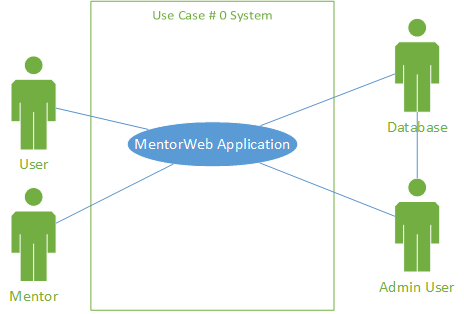
\includegraphics{UseCase0System}

				\begin{tabular}{|p{12 cm}|}
					\hline
					Name: System \\ \hline
					Actors: User, Mentor, Database, Admin User \\ \hline
					Entry Condition: User turns on MentorWeb System \\ \hline
					Flow of Events:
					\begin{enumerate*}
						\item User brings up MentorWeb in their browser
						\item User logs in (see Use Case 1)
					\end{enumerate*} \\ \hline
					Exit condition: User leaves MentorWeb site \\ \hline
					Exceptions: Lost internet connection \\ \hline
				\end{tabular}

				\caption{Use Case Diagram for Use Case 0: System}
				\label{UC0}
            \end{figure}


            \begin{figure}[H]
				\centering
				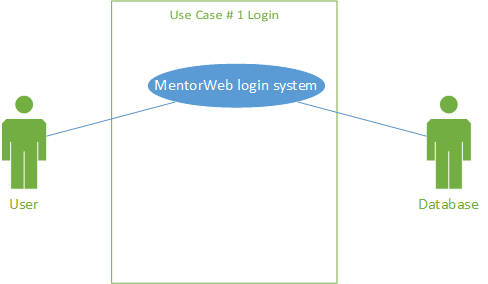
\includegraphics{UseCase1Login}

				\begin{tabular}{|p{12 cm}|}
					\hline
					Name: Login \\ \hline
					Actors: User, Database \\ \hline
					Entry Condition: User has established connection with
					MentorWeb system\\ \hline
					Flow of Events:
					\begin{enumerate*}
						\item User attempts to log into MentorWeb
						\item User either successfully logs in or user
						credentials do not work
					\end{enumerate*} \\ \hline
					Exit condition: User successfully logs in \\ \hline
					Exceptions: User has no account and must register (see Use
					Case 2) \\ \hline
				\end{tabular}

				\caption{Use Case Diagram for Use Case 1: Login}
				\label{UC1}
            \end{figure}

            \begin{figure}[H]
            \centering
            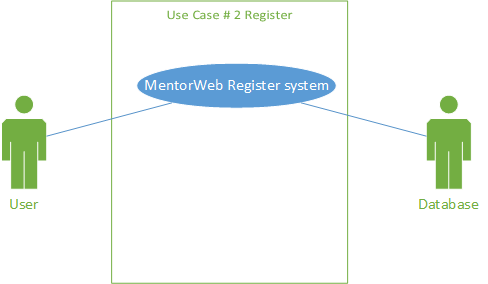
\includegraphics{UseCase2Register}

				\begin{tabular}{|p{12 cm}|}
					\hline
					Name: Register \\ \hline
					Actors: User, Database \\ \hline
					Entry Condition: User is connected to, but does not have an
					account with, the MentorWeb system\\ \hline
					Flow of Events:
					\begin{enumerate*}
						\item User enters in a valid email address to which a
						validation email is sent
						\item User creates a secure password
						\item User enters validation code from validation email
					\end{enumerate*} \\ \hline
					Exit condition: User has successfully created a new account
					\\ \hline
					Exceptions: Account already exists \\ \hline
				\end{tabular}

            \caption{Use Case Diagram for Use Case 2: Register}
            \label{UC2}
            \end{figure}

            \begin{figure}[H]
            \centering
            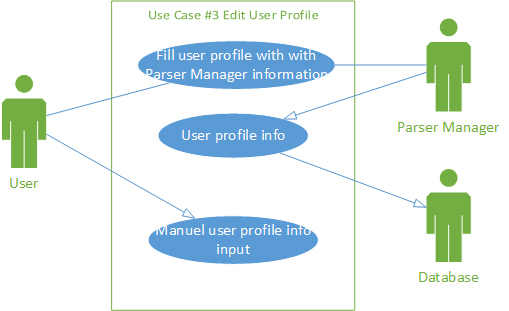
\includegraphics{UseCase3EditUserProfile}

				\begin{tabular}{|p{12 cm}|}
					\hline
					Name: Edit User Profile \\ \hline
					Actors: User, Parse Manager, Database \\ \hline
					Entry Condition: User has logged into MentorWeb system
					\\ \hline
					Flow of Events:
					\begin{enumerate*}
						\item User optionally chooses to import information from
						LinkedIn account to fill user information fields
						\item User edits information fields manually to insert
						or correct information
						\item User submits changes to information
						\item Information is uploaded to the database
					\end{enumerate*} \\ \hline
					Exit condition: Database is updated
					\\ \hline
					Exceptions: Edit is cancelled \\ \hline
				\end{tabular}

            \caption{Use Case Diagram for Use Case 3: Edit User Profile}
            \label{UC3}
            \end{figure}

            \begin{figure}[H]
            \centering
            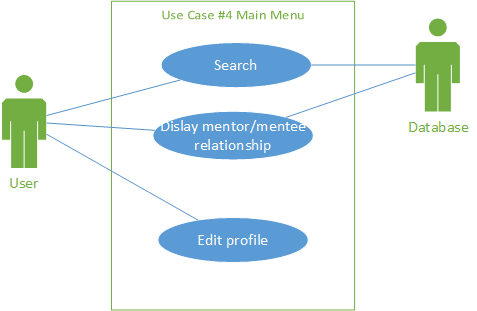
\includegraphics{UseCase4MainMenu}

				\begin{tabular}{|p{12 cm}|}
					\hline
					Name: Main Menu \\ \hline
					Actors: User, Database \\ \hline
					Entry Condition: User has logged into MentorWeb system
					\\ \hline
					Flow of Events:
					\begin{enumerate*}
						\item User MentorWeb network displayed
						\item User has options to search for mentors, view their
						mentor's information, or edit their user profile
					\end{enumerate*} \\ \hline
					Exit condition: User navigates to other MentorWeb components
					\\ \hline
					Exceptions: none \\ \hline
				\end{tabular}

            \caption{Use Case Diagram for Use Case 4: Main Menu}
            \label{UC4}
            \end{figure}

            \begin{figure}[H]
            \centering
            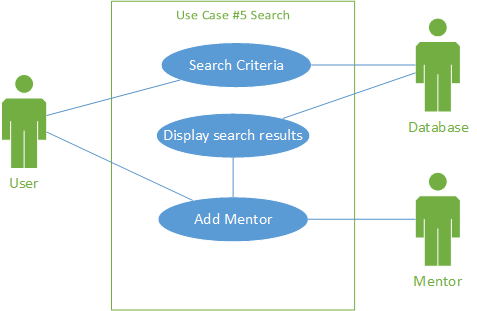
\includegraphics{UseCase5Search}

				\begin{tabular}{|p{12 cm}|}
					\hline
					Name: Search \\ \hline
					Actors: User, Database, Mentor \\ \hline
					Entry Condition: User selects to search for mentors
					\\ \hline
					Flow of Events:
					\begin{enumerate*}
						\item User enters search criteria for mentors they want
						to connect with
						\item System searches database and displays search
						results
						\item User selects which mentors they want to connect
						with
						\item Mentor consents to connection with mentee
					\end{enumerate*} \\ \hline
					Exit condition: Mentor-mentee connection is established
					\\ \hline
					Exceptions: No mentors interesting to the user are found, or
					connection is denied by mentor \\ \hline
				\end{tabular}

            \caption{Use Case Diagram for Use Case 5: Search}
            \label{UC5}
            \end{figure}

            \begin{figure}[H]
            \centering
            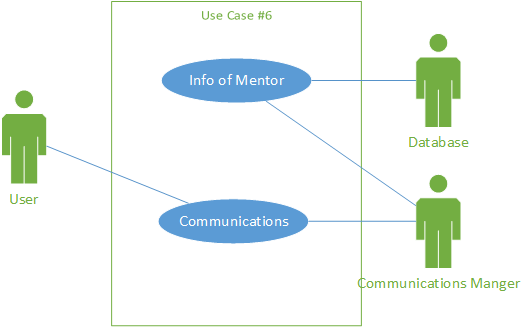
\includegraphics{UseCase6MentoMenteeConnection}

				\begin{tabular}{|p{12 cm}|}
					\hline
					Name: Mentor and Mentee Comunication \\ \hline
					Actors: User, Database, Communications Manager \\ \hline
					Entry Condition: User selects to search for mentors
					\\ \hline
					Flow of Events:
					\begin{enumerate*}
						\item User chooses Mentor to view their information
						\item User selects to contact selected mentor by
						utilizing Communications Manager
					\end{enumerate*} \\ \hline
					Exit condition: Communication occurs
					\\ \hline
					Exceptions: Mentor/Mentee unavailable for communication
					\\ \hline
				\end{tabular}

            \caption{Use Case Diagram for Use Case 6: Mentor-Mentee
			Communication}
            \label{UC6}
            \end{figure}

            \begin{figure}[H]
            \centering
            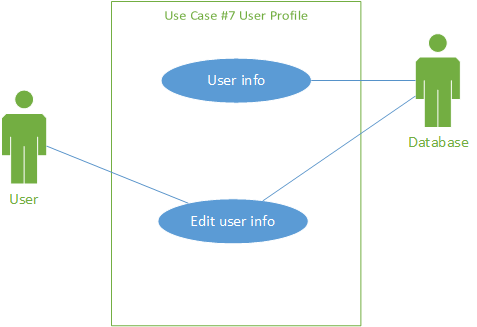
\includegraphics{UseCase7UserProfile}

				\begin{tabular}{|p{12 cm}|}
					\hline
					Name: User Profile
					\\ \hline
					Actors: User, Database
					\\ \hline
					Entry Condition: User logged in to MentorWeb
					\\ \hline
					Flow of Events:
					\begin{enumerate*}
						\item Database displays information about user
						\item User optionally selects to edit their profile
					\end{enumerate*} \\ \hline
					Exit condition: User leaves or begins editing profile
					\\ \hline
					Exceptions: none
					\\ \hline
				\end{tabular}

            \caption{Use Case Diagram for Use Case 7: User Profile}
            \label{UC7}
            \end{figure}

            \begin{figure}[H]
            \centering
            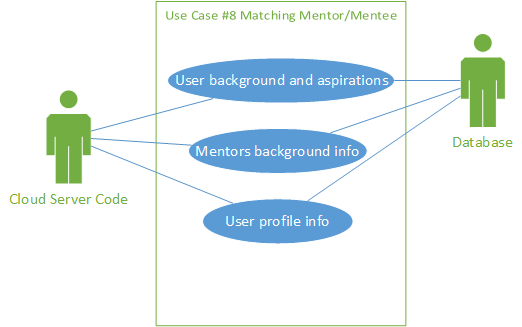
\includegraphics{UseCase8MatchingMentorMentee}

				\begin{tabular}{|p{12 cm}|}
					\hline
					Name: Matching Mentor with Mentee
					\\ \hline
					Actors: Cloud Server Code, Database
					\\ \hline
					Entry Condition: User has entered their background
					information and aspirations
					\\ \hline
					Flow of Events:
					\begin{enumerate*}
						\item Cloud Server Code parses through user's background
						and aspiration information for keywords
						\item Cloud Server Code parses through background
						information from list of Mentors based on parsed user
						information
						\item Cloud Server Code matches user background and
						aspiration information with Mentor's background
						information
						\item Cloud Server Code sends luser list of recommended
						Mentors
					\end{enumerate*} \\ \hline
					Exit condition: Cloud Server Code makes recommendations to
					user
					\\ \hline
					Exceptions: No applicable matches
					\\ \hline
				\end{tabular}

            \caption{Use Case Diagram for Use Case 8: Cloud Matching}
            \label{UC8}
            \end{figure}

        \subsubsection{Object Model}
			\begin{figure}[H]
				\centering
				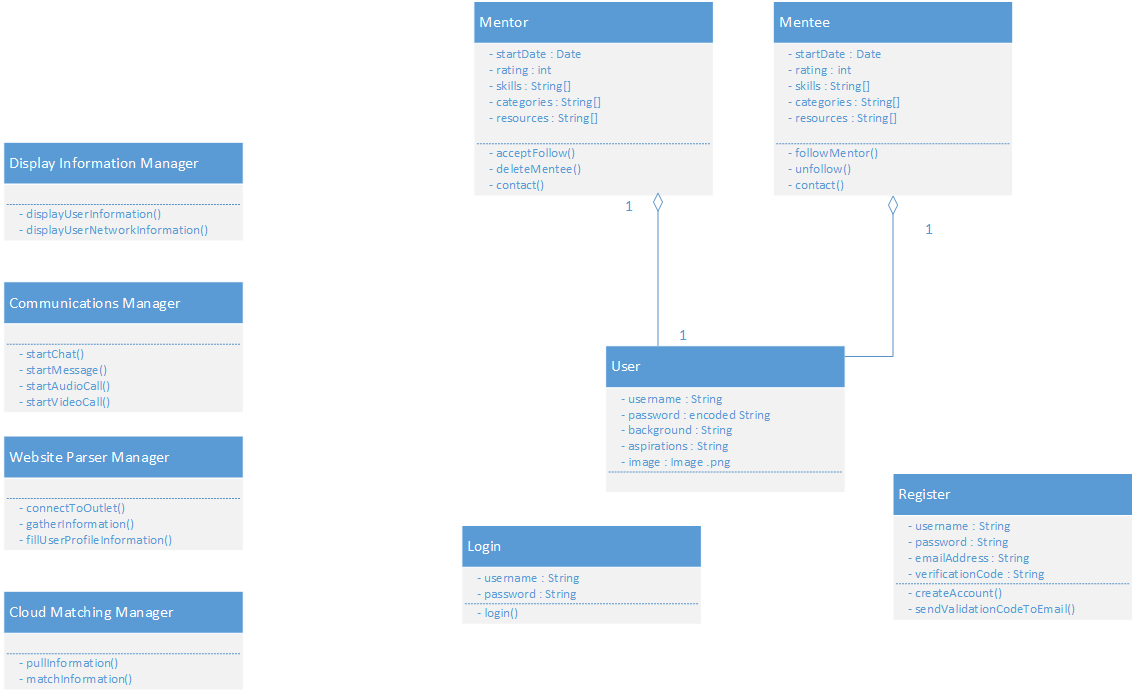
\includegraphics[angle=90,width=10 cm]{ClassDiagram}
				\caption{Class Diagram for MentorWeb}
				\label{ClassD}
			\end{figure}

        \subsubsection{Dynamic Model}

            \begin{figure}[H]
            \centering
            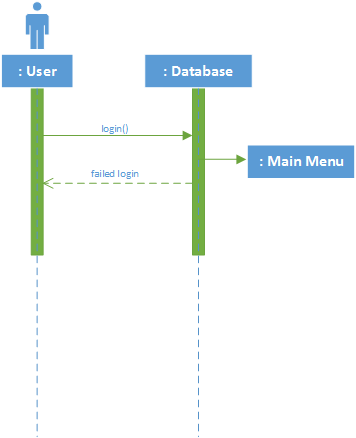
\includegraphics{SequenceUseCase1Login}
            \caption{Sequence Diagram for Use Case 1: Login}
            \label{SUC1}
            \end{figure}

            \begin{figure}[H]
            \centering
            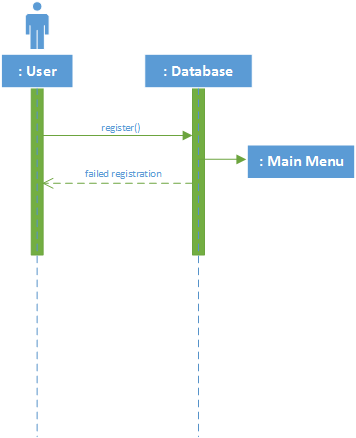
\includegraphics{SequenceUseCase2Register}
            \caption{Sequence Diagram for Use Case 2: Register}
            \label{SUC2}
            \end{figure}

            \begin{figure}[H]
            \centering
            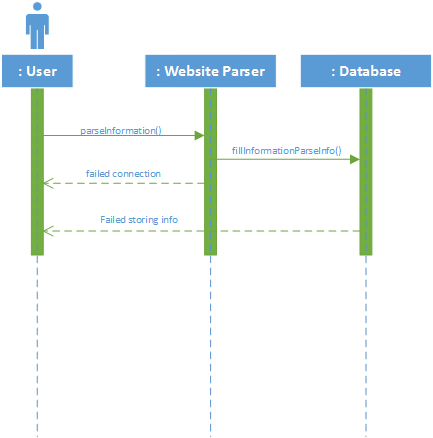
\includegraphics{SequenceUseCase3EditUserProfile}
            \caption{Sequence Diagram for Use Case 3: Edit User Profile}
            \label{SUC3}
            \end{figure}

            \begin{figure}[H]
            \centering
            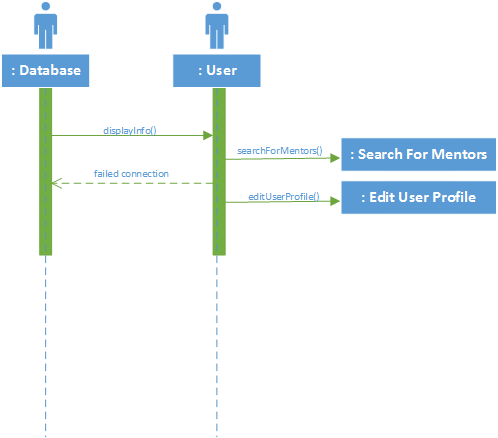
\includegraphics{SequenceUseCase4MainMenu}
            \caption{Sequence Diagram for Use Case 4: Main Menu}
            \label{SUC4}
            \end{figure}

            \begin{figure}[H]
            \centering
            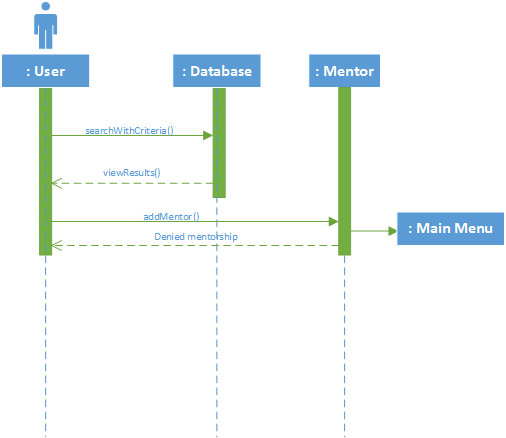
\includegraphics{SequenceUseCase5Search}
            \caption{Sequence Diagram for Use Case 5: Search}
            \label{SUC5}
            \end{figure}

            \begin{figure}[H]
            \centering
            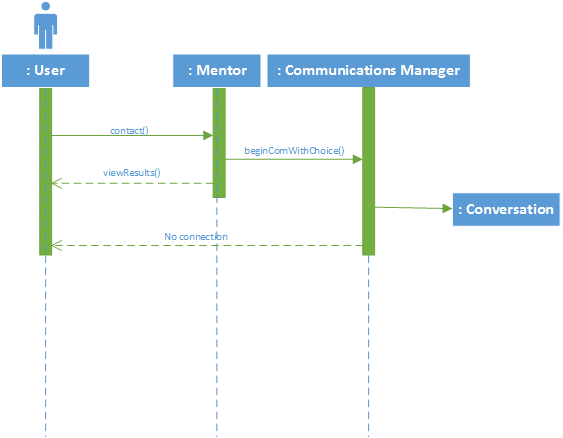
\includegraphics{SequenceUseCase6Communication}
            \caption{Sequence Diagram for Use Case 6: Communication}
            \label{SUC6}
            \end{figure}

            \begin{figure}[H]
            \centering
            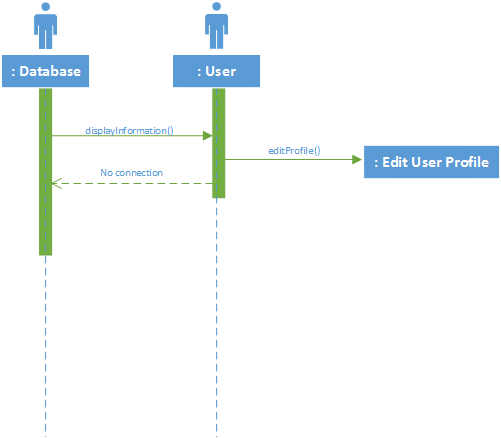
\includegraphics{SequenceUseCase7UserProfile}
            \caption{Sequence Diagram for Use Case 7: User Profile}
            \label{SUC7}
            \end{figure}

            \begin{figure}[H]
            \centering
            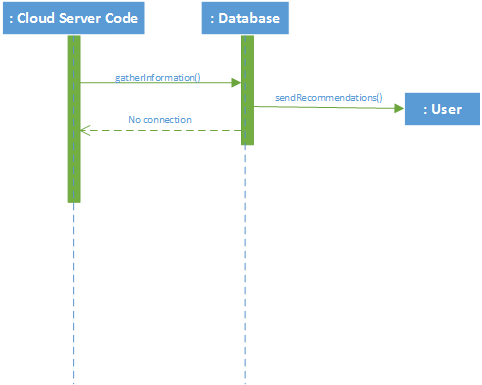
\includegraphics{SequenceUseCase8CloudMatching}
            \caption{Sequence Diagram for Use Case 8: Cloud Matching}
            \label{SUC8}
            \end{figure}

        \subsubsection{User Interface}
			\begin{figure}[H]
				\centering
				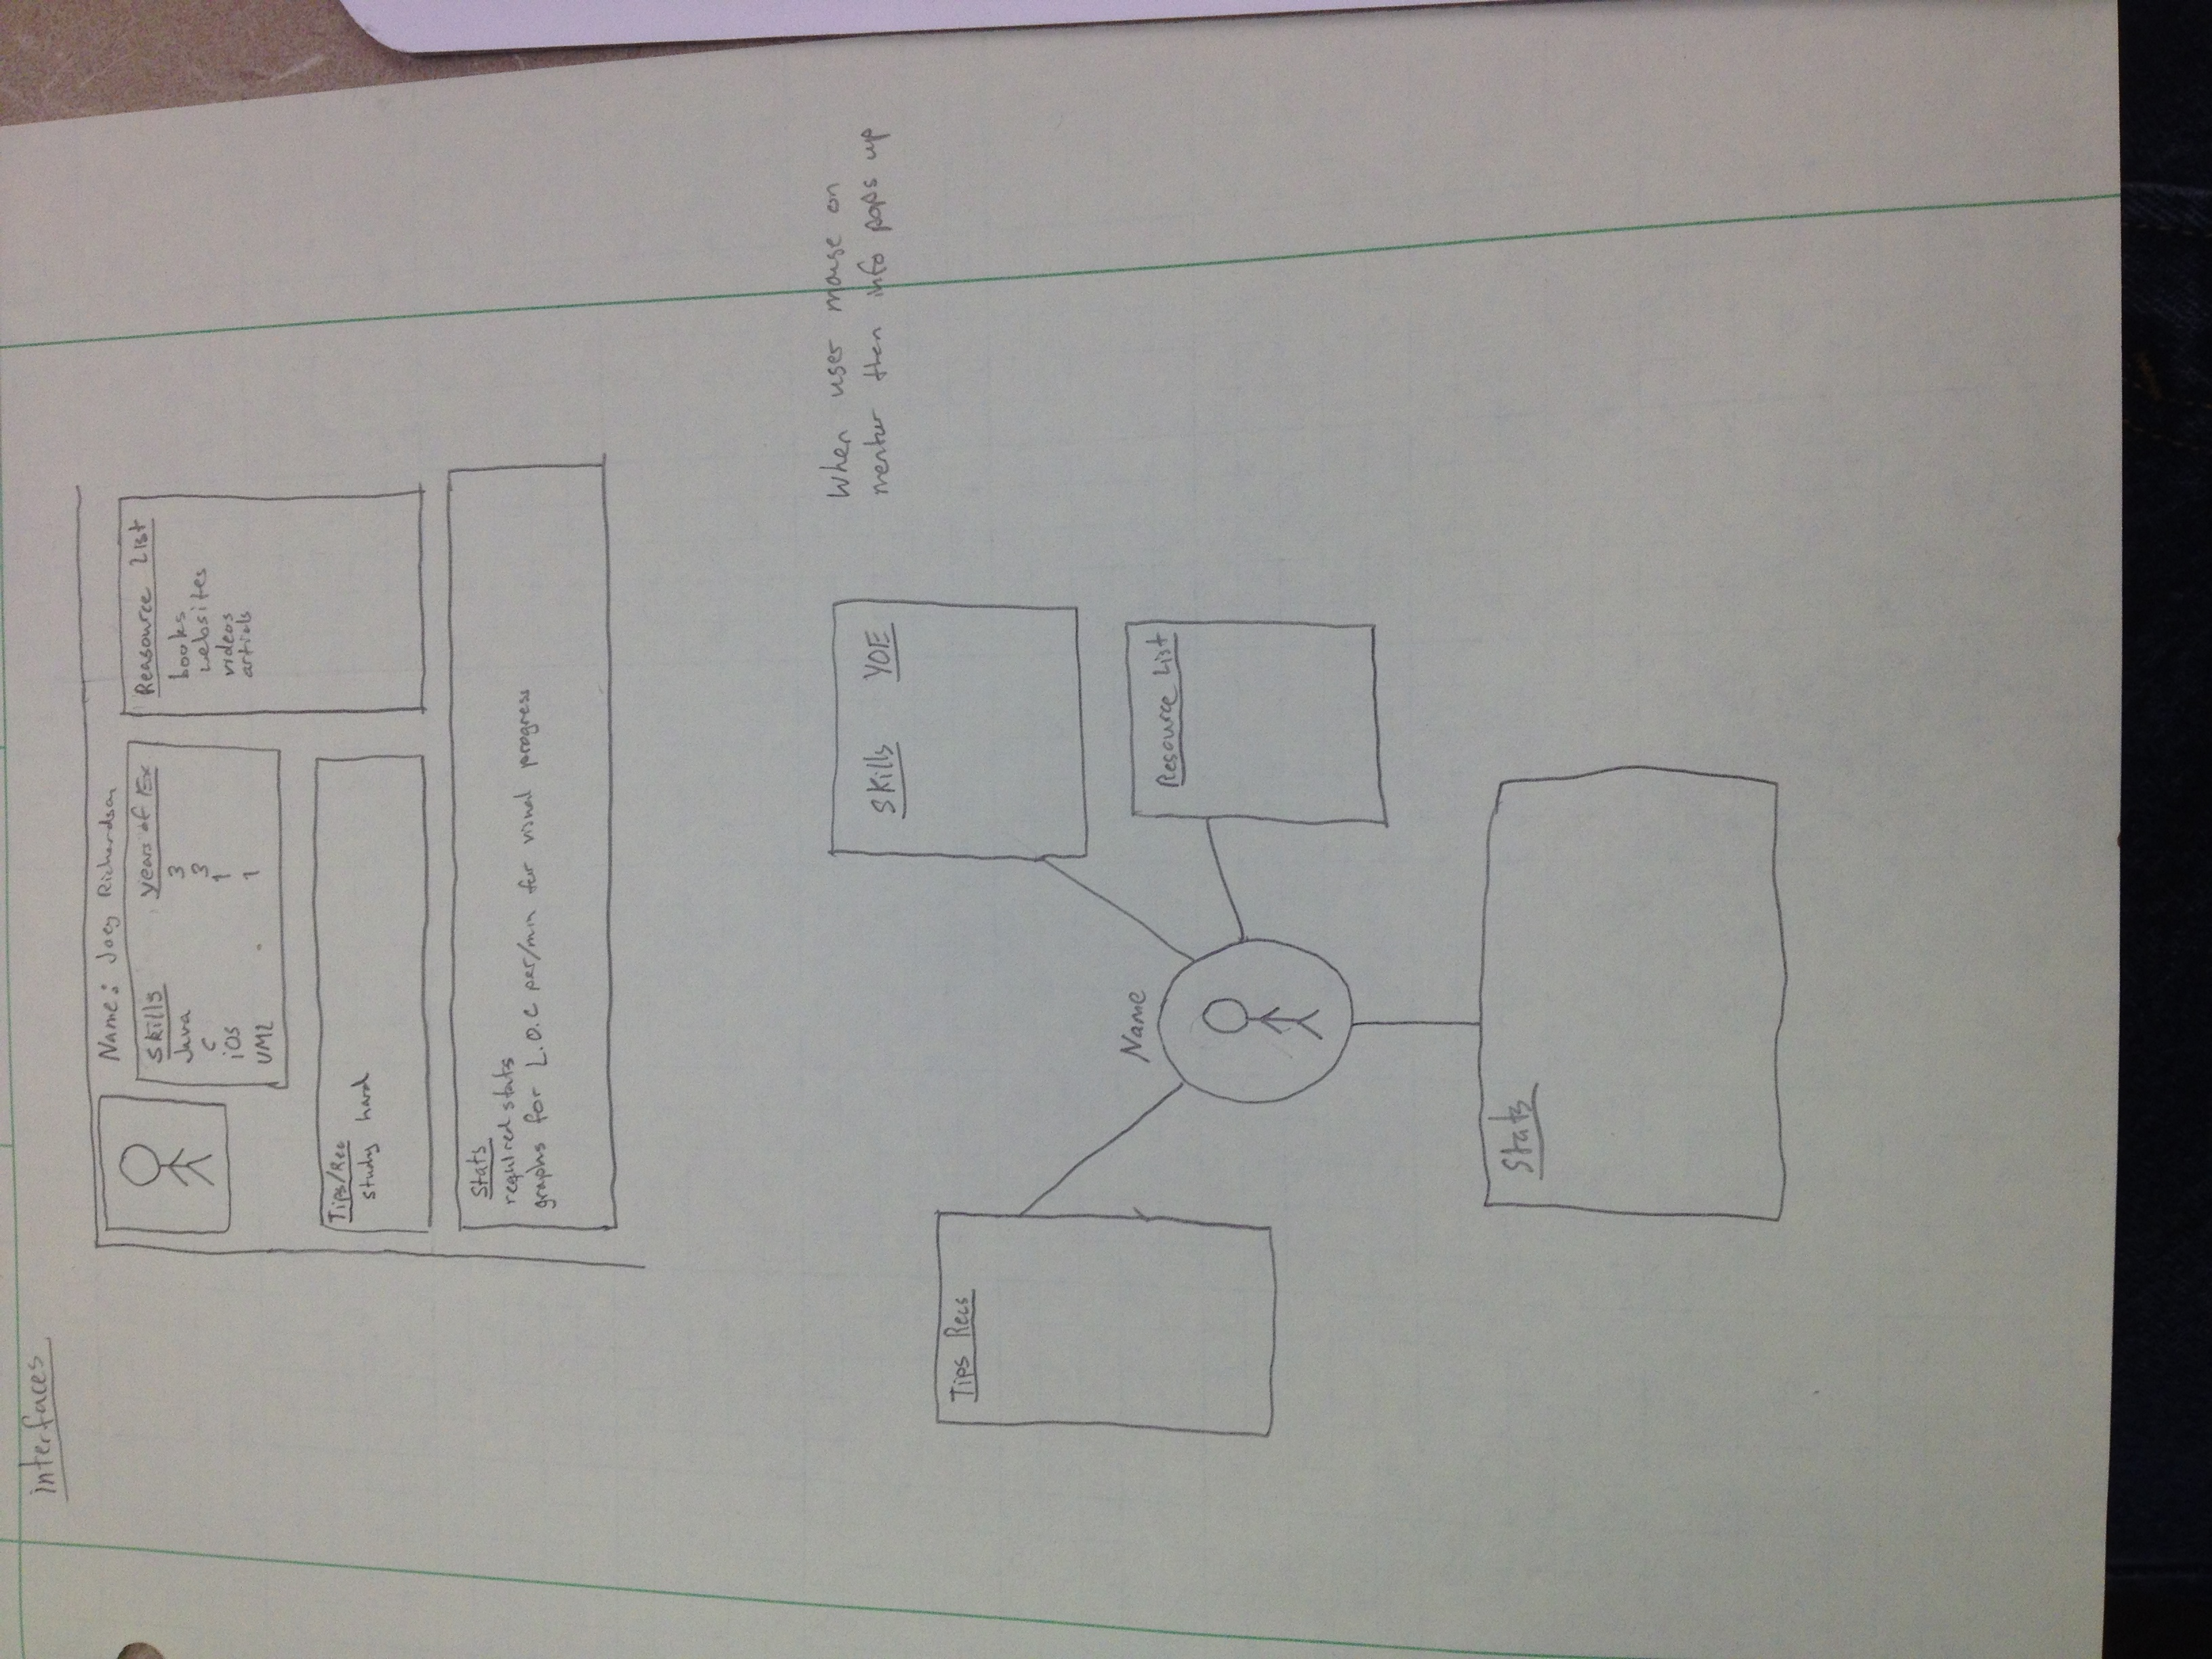
\includegraphics[angle=-90,width=12 cm]{PossibleUserInterface}
				\caption{Mockup of a possible user interface}
				\label{UIMockup}
			\end{figure}

			\begin{figure}[H]
				\centering
				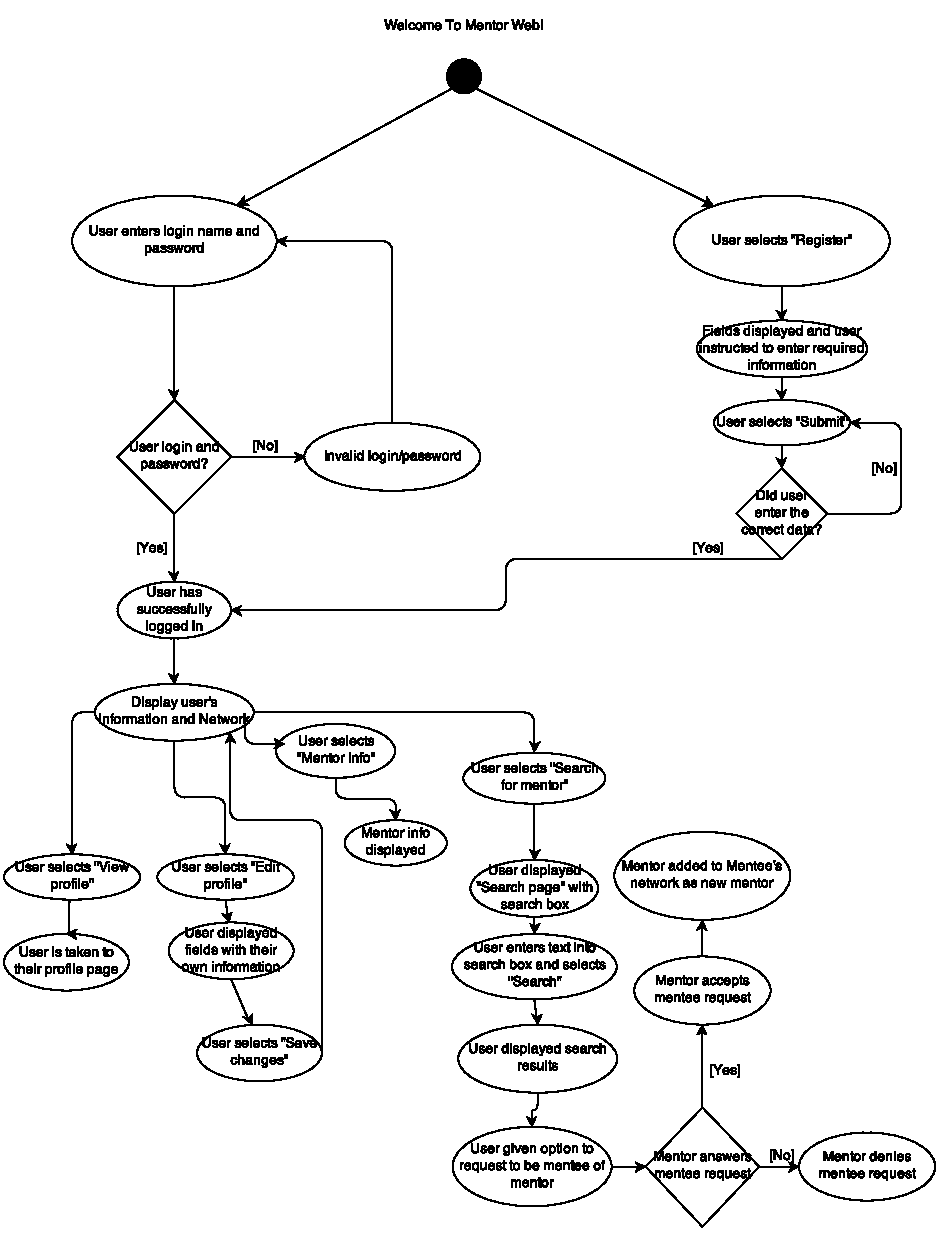
\includegraphics[width=12 cm]{Activity_Diagram}
				\caption{Activity Diagram}
				\label{ActivityD}
			\end{figure}

			\begin{figure}[H]
				\centering
				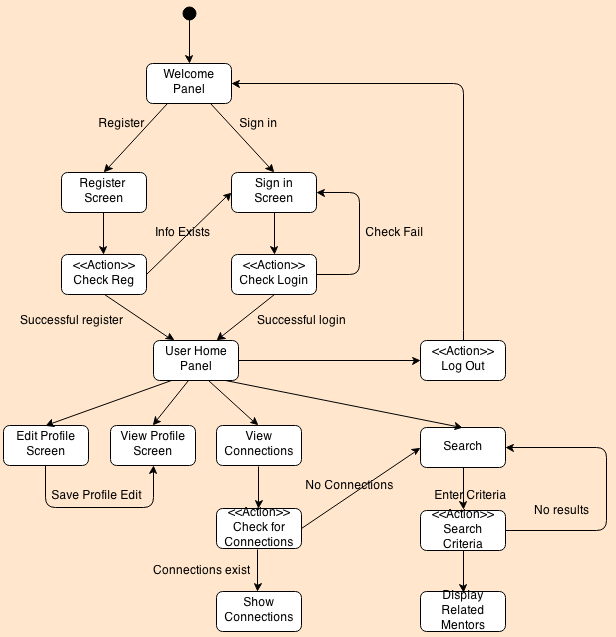
\includegraphics[width=12 cm]{State_Diagram}
				\caption{State Diagram}
				\label{StateD}
			\end{figure}

			\begin{figure}[H]
				\centering
				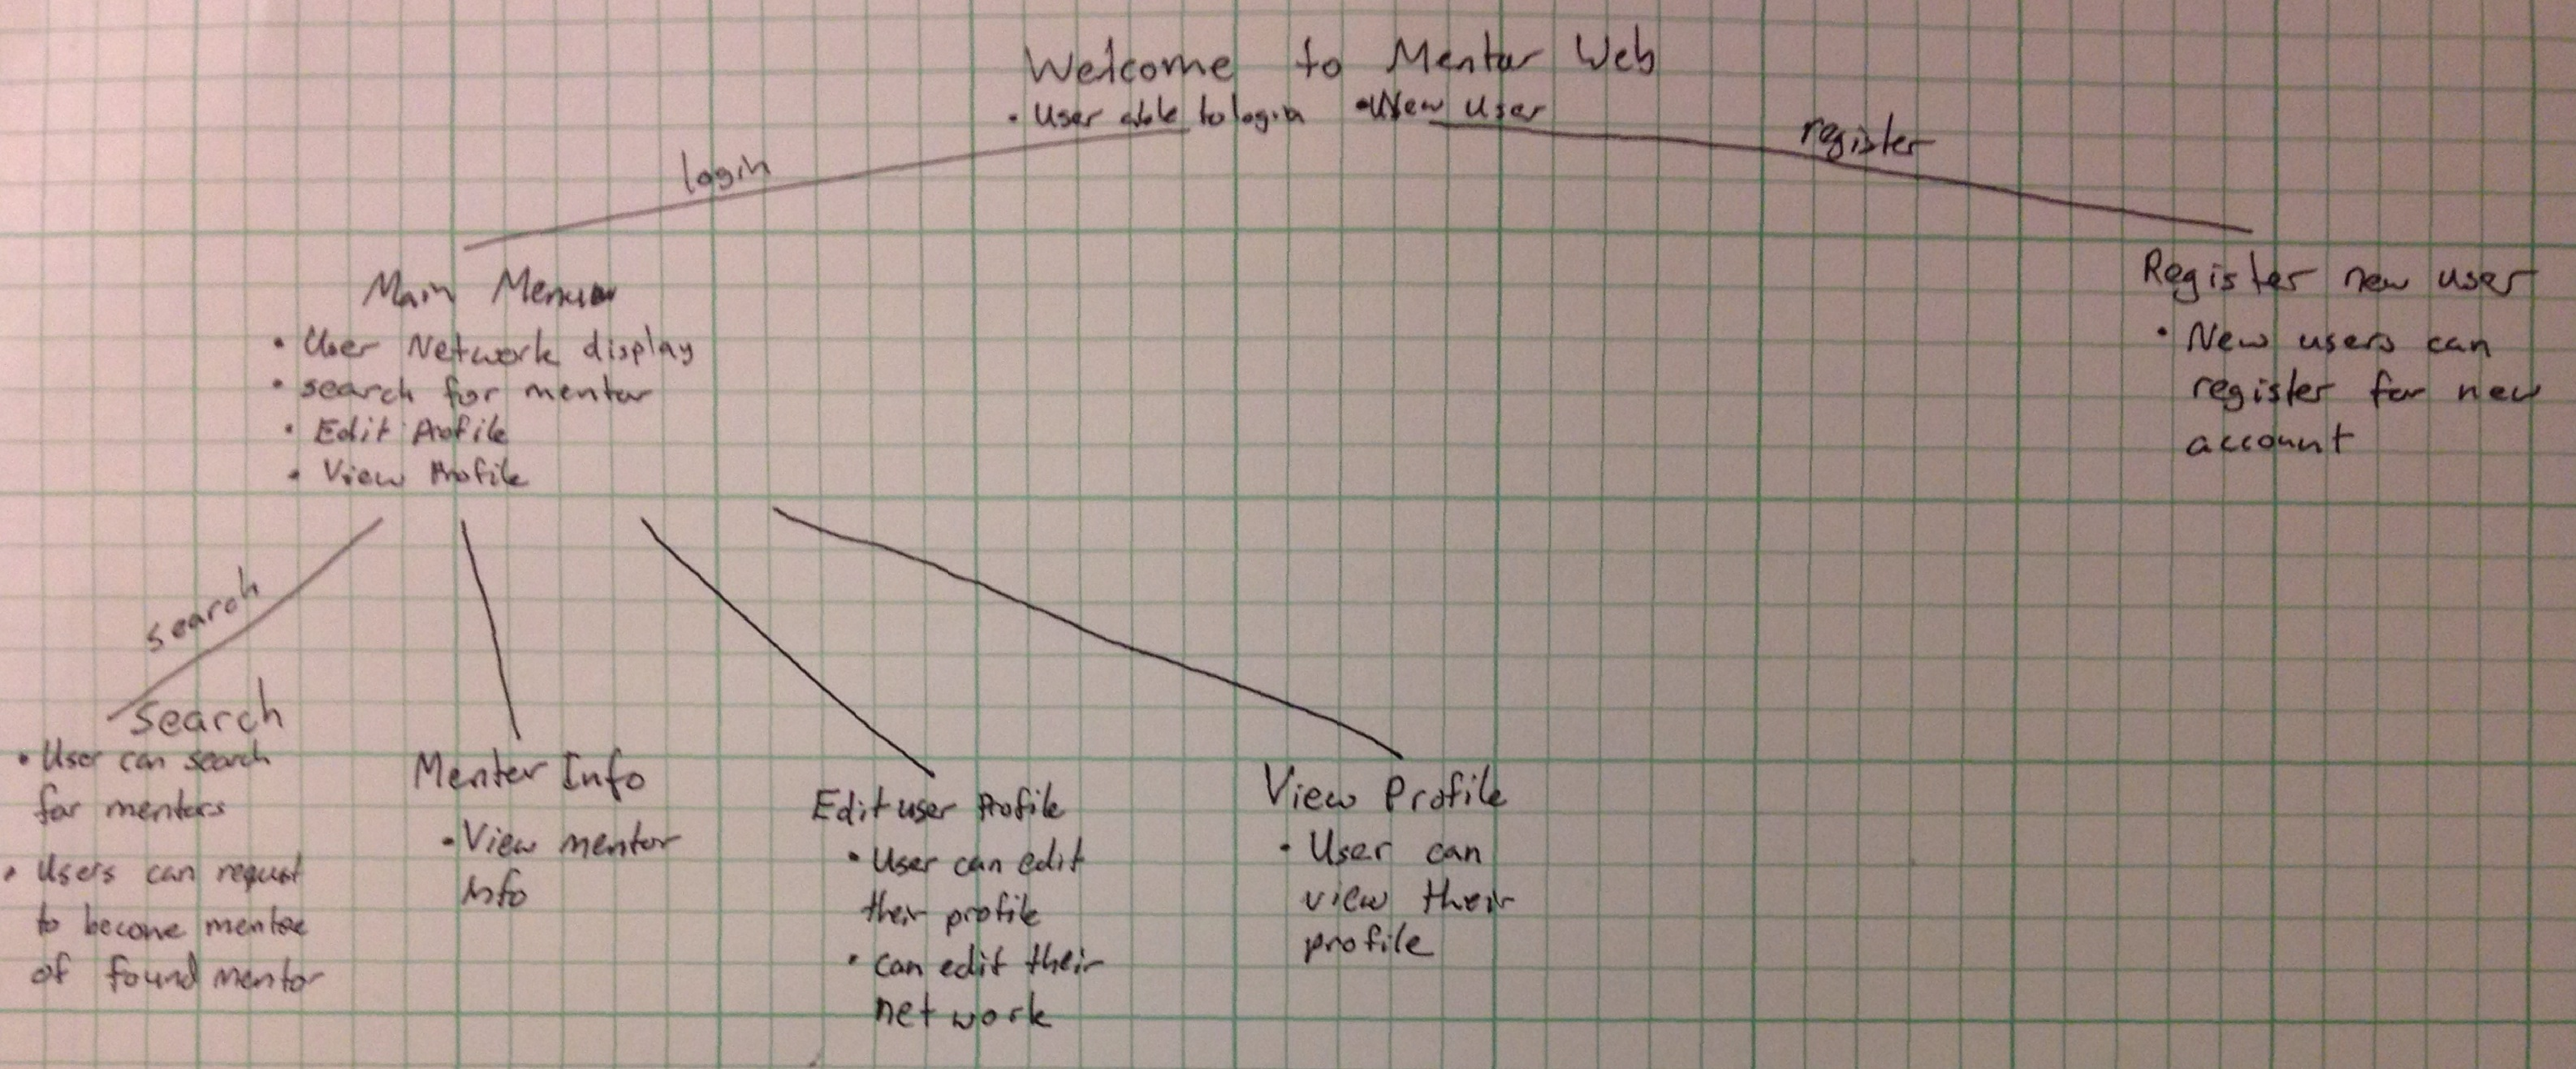
\includegraphics[width=12 cm]{Nav_mentor_web}
				\caption{Mentor Web Navigation}
				\label{NavD}
			\end{figure}

% TODO
\section{Glossary}

% TODO
\section{Appendices}

    % TODO
    \subsection{Hardware Requirements}

    % TODO
    \subsection{Project Plan}

    % TODO
    \subsection{Team Staffing and Responsibilities}

    % TODO
    \subsection{Notebook Log}

    % TODO
    \subsection{Index}
    \printindex
    

\end{document}
